% -*- coding:utf-8 -*-
\documentclass{standalone}
\usepackage[UTF8]{ctex}
\usepackage{tikz}
\usepackage{amsmath}
\usetikzlibrary{matrix,calc,shapes,backgrounds,patterns,positioning,decorations.pathreplacing}
\begin{document}
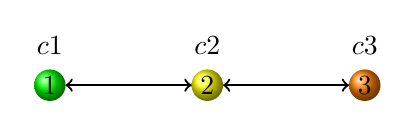
\begin{tikzpicture}
[
vertex1/.style={shading=ball, ball color=green},
vertex2/.style={shading=ball, ball color=yellow},
vertex3/.style={shading=ball, ball color=orange},
]
\shade[vertex1] (0,0) circle (0.2) node {$1$} node at (0,0.5) {$c1$};
\shade[vertex2] (2, 0) circle (0.2) node {$2$} node at (2,0.5) {$c2$};
\shade[vertex3] (4, 0) circle (0.2) node {$3$} node at (4,0.5) {$c3$};
\draw[thick, <->] (0.2,0) -- (1.8,0);
\draw[thick, <->] (2.2,0) -- (3.8, 0);
\end{tikzpicture}
\end{document}